\section{Experiments}
We conduced several experiments to measure the soundness of our solution. Since the parallel message processing gives the better performance, we present details of those experiments with distributed setup as well a singel JVM setup. All these experiments were performed on a LAN with a network bandwidth of 1Gbps and all machines were Intel(R) Xeon(R) 2.4GHz, 4 core duo machines with 16 GB of memory. 

\subsection{Frequent routes query}

\begin{figure}[!t]
        \centering
        \includegraphics[width=3.0in]{routegraph.png}
        \caption{Process graph to evaluate top ten frequent routes.}
        \label{routegraph}
\end{figure}

Figure \ref{routegraph} shows the process graph used to process frequent route queries. \textit{RouteEventEmitter} reads the data file and emits events with a sequence number. \textit{RouteEmitter} contains a set of threads (equals to the number of \textit{RouteProcessors}) to emit events more efficiently. When processing each line first it reads the data line and creates a Route object using longitude and latitude coordinates of pickup and dropoff locations. Then it distributes the events among the \textit{RouteProcessors} using the hash value of the Route object. \textit{TopRouteProcessor} aggregates the results and saves them to a file.

We deployed this process graph to a distributed stream processing system we have developed, and  measured the execution time and the average message latency varying the number of route processors with the data set given (173 million records). In local set up, we use a new thread to execute a new instance and in distributed setup we add a new node to execute the new instance.

\begin{figure}[!t]
        \centering
        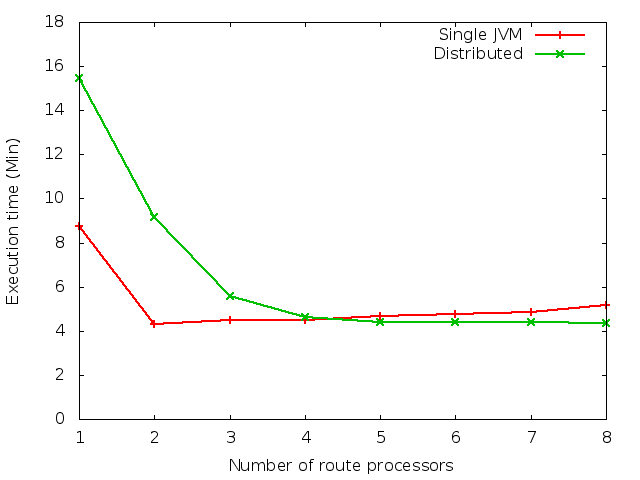
\includegraphics[width=3.0in]{time_route.png}
        \caption{Execution times to evaluate top ten frequent routes.}
        \label{time_route}
\end{figure}
 
Figure \ref{time_route} shows the execution times. For both setups execution time is higher for single instance due to lack of parallelism of the system. For distributed setup time get reduced with addition of new nodes and comes to a constant level. This means our solution scales up to 4 node level and maintains a constant throughput. This is due to two reasons. Firstly, \textit{RouteProcessor} is not a computing intensive process. Secondly, there is only one \textit{RouteEventEmitter} and the speed at which it can read and send messages becomes the bottleneck. For single JVM set up highest throughput is achieved with two route processors. After that point time get slightly increases due to context switching.

\begin{figure}[!t]
        \centering
        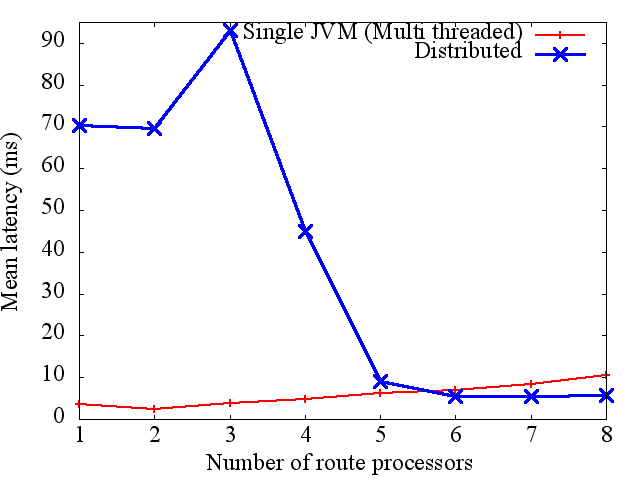
\includegraphics[width=3.0in]{latency_route.png}
        \caption{Latencies to evaluate top ten frequent routes.}
        \label{latency_route}
\end{figure}


Figure \ref{latency_route} shows the latencies. For single JVM setup latency get reduced at 2 and slightly get increase due to context switching as in the execution times. For distributed set up initial latency is high due to communication and message serialization parsing overheads. With higher number of processors latency get reduced.

\subsection{Profitable cells query}

\begin{figure}[!t]
        \centering
        \includegraphics[width=3.0in]{profictgraph.png}
        \caption{Process graph to evaluate top ten profitable cells.}
        \label{profictgraph}
\end{figure}

Figure \ref{profictgraph} shows the process graph for profitable cells query. \textit{ProfitEventEmitter} reads the data file and calculates the pickup cell and dropoff cell details using longitude and latitude coordinates. Then it creates two events one for dropoff part and other to pickup part, with different sequence numbers and distributes the events among \textit{ProfictCalculators} using the hash value of the cell. In this way cells are partitioned into different \textit{ProfitCalculator} instances and each instance gets all the events relevant to its' cell set. We use a set of threads (equals to the number of Profict Calculators) to emit data as in the previous query. Finally \textit{TopProfictProcessor} aggregates events and writes to a file. 
Similar to earlier experiment,  we deployed this process graph to our system and measured the execution time and the average message latency with the data set given for both single JVM setup and distributed setup.


\begin{figure}[!t]
        \centering
        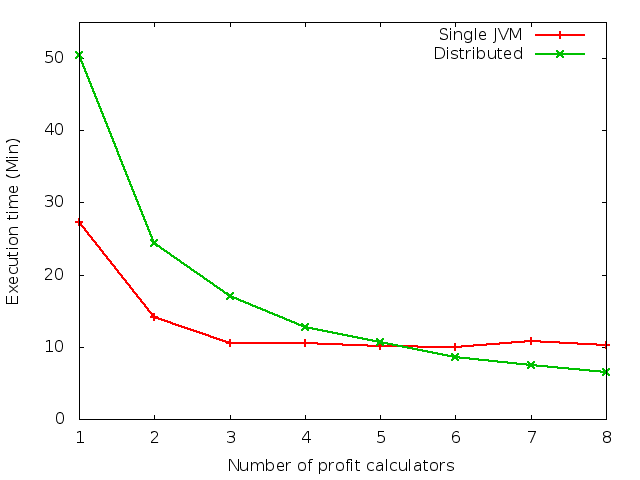
\includegraphics[width=3.0in]{time_profit.png}
        \caption{Execution times to evaluate top ten profitable cells.}
        \label{time_profit}
\end{figure}
 
Figure \ref{time_profit} shows the execution times for both setups. In both setups, there is a higher latency at one instance due to lack of parallelism. Then for distributed set up execution times get reduced with addition of new resources and for single JVM setup it remains a constant. This shows our solution scales up in a distributed setup. We can increase the system throughput by adding new nodes until \textit{ProfitEventEmitter} becomes the bottleneck.


\begin{figure}[!t]
        \centering
        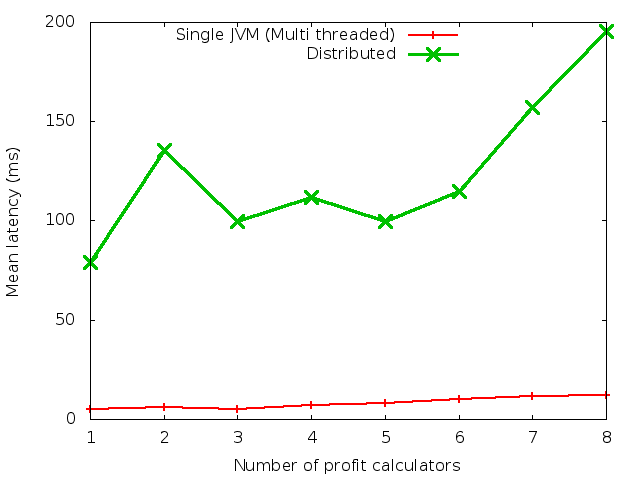
\includegraphics[width=3.0in]{latency_profit.png}
        \caption{Latencies to evaluate top ten profitable cells.}
        \label{latency_profit}
\end{figure}

Figure \ref{latency_profit} shows the latencies. For single JVM, latencies slightly increased with the addition of new instances as expected. But for distributed setups there is a higher latencies compared to others. This latency is due to longer queues at the \textit{TopProfitProcessor}. In our message ordering process, we can only send a message to \textit{TopProfitProcessor} only if all queues are not empty. This allows some processes with less top ten profitable events to delay other process messages. This problem can  possibly fixed by adding a limit to the message queue size. On the other hand in a real time system, this event ordering many not required since event processing happens at real time. 



